\documentclass[11pt,a4paper]{article}
\usepackage[utf8]{inputenc}
\usepackage[T1]{fontenc}
\usepackage{amsmath,amssymb}
\usepackage{booktabs}
\usepackage{graphicx}
\usepackage{hyperref}
\usepackage{multirow}
\usepackage{xcolor}
\usepackage[margin=1in]{geometry}
\usepackage{enumitem}
\usepackage{subcaption}

% Figures live in ../reports/figures relative to this file (paper/).
\graphicspath{{../reports/figures/}}

\title{A Computational Study of Disagreement-Aware Fusion,\\
Calibration, and Resampling Inference\\
in Text and Metadata Classification}
\author{Krish Jain \\
  PSTAT 232: Computational Techniques in Statistics \\
  Department of Statistics \& Applied Probability \\
  University of California, Santa Barbara}
\date{}

\begin{document}
\maketitle

\begin{abstract}
This project is a computational-statistics study of a binary text--metadata
classification problem in which the two modalities frequently \emph{disagree}.
Rather than treating the task purely as a machine-learning benchmark, we frame
it around four computational themes that recur in modern statistics:
(i) \emph{empirical risk minimization} (ERM) and a reweighted, disagreement-aware
variant; (ii) \emph{post-hoc calibration} and uncertainty quantification through
temperature scaling, including a new \emph{group-conditional} estimator driven by
an inference-time conflict proxy; (iii) \emph{resampling inference}---nonparametric
bootstrap confidence intervals and paired bootstrap / McNemar tests---to attach
honest sampling uncertainty to every reported metric; and (iv) a
\emph{leakage-controlled evaluation protocol} that removes a label-encoding
product-level aggregate from the primary pipeline. On the Amazon Reviews 2023
\texttt{All\_Beauty} category, the leakage-controlled fusion model attains
$0.876$ test accuracy ($95\%$ bootstrap CI $[0.864,0.888]$) but is statistically
\emph{indistinguishable} from a text-only model (paired bootstrap $p=0.42$,
McNemar $p=0.42$), while removing the leaky feature collapses the metadata
model from $0.687$ to $0.566$ accuracy. Group-conditional calibration gives a
small but consistent reduction in non-conflict calibration error; importantly,
once leakage is controlled the dramatic conflict-driven miscalibration reported
under the leaky setup is much milder---itself a computational finding about how
data leakage manufactures apparent pathology. All numbers in this report are
produced by the accompanying reproducible scripts; none are hand-entered.
\end{abstract}

\tableofcontents

\section{Introduction}
\label{sec:intro}

Multimodal classifiers combine heterogeneous inputs---here, review \emph{text}
and structured \emph{metadata}---under the assumption that more information
yields better decisions. In practice the modalities often conflict: a review may
read positively while its star-derived label is negative. This project asks a
sequence of \emph{statistical} questions about that conflict regime, rather than
a single ``which model wins'' question:

\begin{enumerate}[leftmargin=*,nosep]
  \item How does the empirical risk of each model decompose across agreement and
        graded-disagreement subpopulations, and does reweighting the ERM
        objective toward disagreement cases change that decomposition?
  \item Is the fusion model's apparent advantage statistically real once we
        attach resampling-based uncertainty, or is it within sampling noise?
  \item Is miscalibration homogeneous across the input space, or does it
        concentrate in the conflict region---and can a \emph{group-conditional}
        post-hoc calibrator exploit a cheap, label-free conflict proxy?
  \item How much of the metadata model's measured skill is an artifact of
        \emph{label leakage} through a product-level rating aggregate?
\end{enumerate}

Our emphasis throughout is on \emph{computational technique}: ERM and reweighted
ERM as optimization problems, temperature scaling as a one-parameter convex
calibration fit, the bootstrap and paired bootstrap as Monte-Carlo inference
procedures, and a leakage-controlled protocol as an experimental-design control.
Every figure and table in this report is produced by the accompanying
reproducible scripts (Section~\ref{sec:repro}).

\section{Statistical Problem Formulation}
\label{sec:formulation}

Let $(X, M, Y)$ denote a review with text features $X \in \mathbb{R}^{d_t}$
(384-dimensional sentence-transformer embeddings), metadata features
$M \in \mathbb{R}^{d_m}$, and binary label $Y \in \{0,1\}$ derived from the star
rating ($Y=1$ if rating $\geq 4$, $Y=0$ if rating $\leq 2$; neutrals dropped).
A model is a map $f_\theta$ producing $\hat p = \mathbb{P}_\theta(Y=1\mid \cdot)$,
hard prediction $\hat y = \mathbf{1}\{\hat p \geq 0.5\}$, and confidence
$c = \max(\hat p, 1-\hat p)$.

\paragraph{Empirical risk.}
Training minimizes the regularized empirical cross-entropy risk
\[
\hat R(\theta) = \frac{1}{n}\sum_{i=1}^{n} w_i\,
\ell\!\left(f_\theta(x_i,m_i),\, y_i\right),
\qquad
\ell(\hat p, y) = -\big[y\log \hat p + (1-y)\log(1-\hat p)\big],
\]
with $w_i \equiv 1$ for standard ERM. The \emph{disagreement-aware} variant sets
$w_i = \omega$ (we use $\omega=5$) on training examples flagged as
text--rating conflicts and $w_i=1$ otherwise, shifting the risk's mass toward the
hard subpopulation.

\paragraph{Disagreement as a latent stratification.}
A pretrained sentiment model produces a text-sentiment label $s_i$ and confidence
$q_i$. We define agreement status $A_i = \mathbf{1}\{s_i = y_i\}$ and a graded
severity using $q_i$ (weak $<0.70 \leq$ medium $<0.90 \leq$ strong). This induces
a stratification of the test population over which we evaluate
\emph{conditional} risk and calibration. Crucially, $s_i$ is a proxy: the
disagreement subset is enriched for genuinely hard or mislabeled reviews, which
we treat as a limitation rather than ground truth.

\paragraph{Targets of inference.}
For each model and each subpopulation $G$ we estimate accuracy
$\alpha_G$, $F_1$, AUROC, expected calibration error (ECE), Brier score, and
negative log-likelihood (NLL). Each is a functional of the unknown joint
distribution estimated on a finite test sample; Section~\ref{sec:results}
attaches sampling uncertainty by resampling that test sample.

\section{Data and Leakage Audit}
\label{sec:data}

We use the Amazon Reviews 2023 corpus (McAuley Lab), \texttt{All\_Beauty}
category, as the primary materialized dataset; four additional categories
(\texttt{Appliances}, \texttt{Digital\_Music}, \texttt{Gift\_Cards},
\texttt{Video\_Games}) are available for sensitivity analysis. The canonical pool
is a class-balanced sample of $20{,}000$ reviews with cached sentence-transformer
embeddings and a precomputed sentiment proxy; a stratified $70/15/15$ split
(seed $42$) yields $14{,}000 / 3{,}000 / 3{,}001$ train/validation/test examples.
On the test split, $2317/20000 \approx 11.6\%$ of pooled reviews are conflicts,
and the disagreement subset has $n=368$ test reviews.

\paragraph{Leakage audit and control.}
The metadata feature set includes \texttt{product\_average\_rating},
a \emph{product-level} aggregate of star ratings. Because the label $Y$ is itself
derived from the per-review rating, this aggregate partially encodes the label
and is a textbook source of target leakage. Our \textbf{primary PSTAT 232
pipeline removes} \texttt{product\_average\_rating} and the prior-driven
\texttt{product\_rating\_number}; the full (leaky) feature set is retained only as
the sensitivity experiment in Table~\ref{tab:leakage}. The leakage-controlled
metadata feature set is therefore
$\{$review length (words, chars), helpful votes, verified purchase, price,
review year$\}$.

\begin{table}[t]
\centering
\caption{Leakage ablation on the \texttt{All\_Beauty} test set: effect of
including the label-encoding \texttt{product\_average\_rating} (full) versus
removing it (leakage-controlled, LC). Removing it collapses the metadata model
but barely changes fusion accuracy---fusion skill is text-driven---while the leaky
feature \emph{worsens} fusion calibration (ECE).}
\label{tab:leakage}
\begin{tabular}{llrrrr}
\toprule
Model & Feature set & Accuracy & AUROC & ECE & Disagree.\ acc. \\
\midrule
Metadata-only & Leakage-controlled & 0.566 & 0.600 & 0.050 & 0.500 \\
Metadata-only & Full (leaky)       & 0.687 & 0.755 & 0.028 & 0.630 \\
Multimodal    & Leakage-controlled & 0.876 & 0.947 & 0.026 & 0.649 \\
Multimodal    & Full (leaky)       & 0.878 & 0.953 & 0.062 & 0.660 \\
\bottomrule
\end{tabular}
\end{table}

The audit (Figure~\ref{fig:leakage}) is itself a computational-statistics result:
the leaky aggregate inflates metadata AUROC by $+0.155$ and accuracy by
$+12$~percentage points, but contributes almost nothing to fusion accuracy while
\emph{tripling} fusion ECE ($0.026 \to 0.062$). Reported metadata ``skill'' under
the full set is thus largely a leakage artifact.

\begin{figure}[t]
\centering
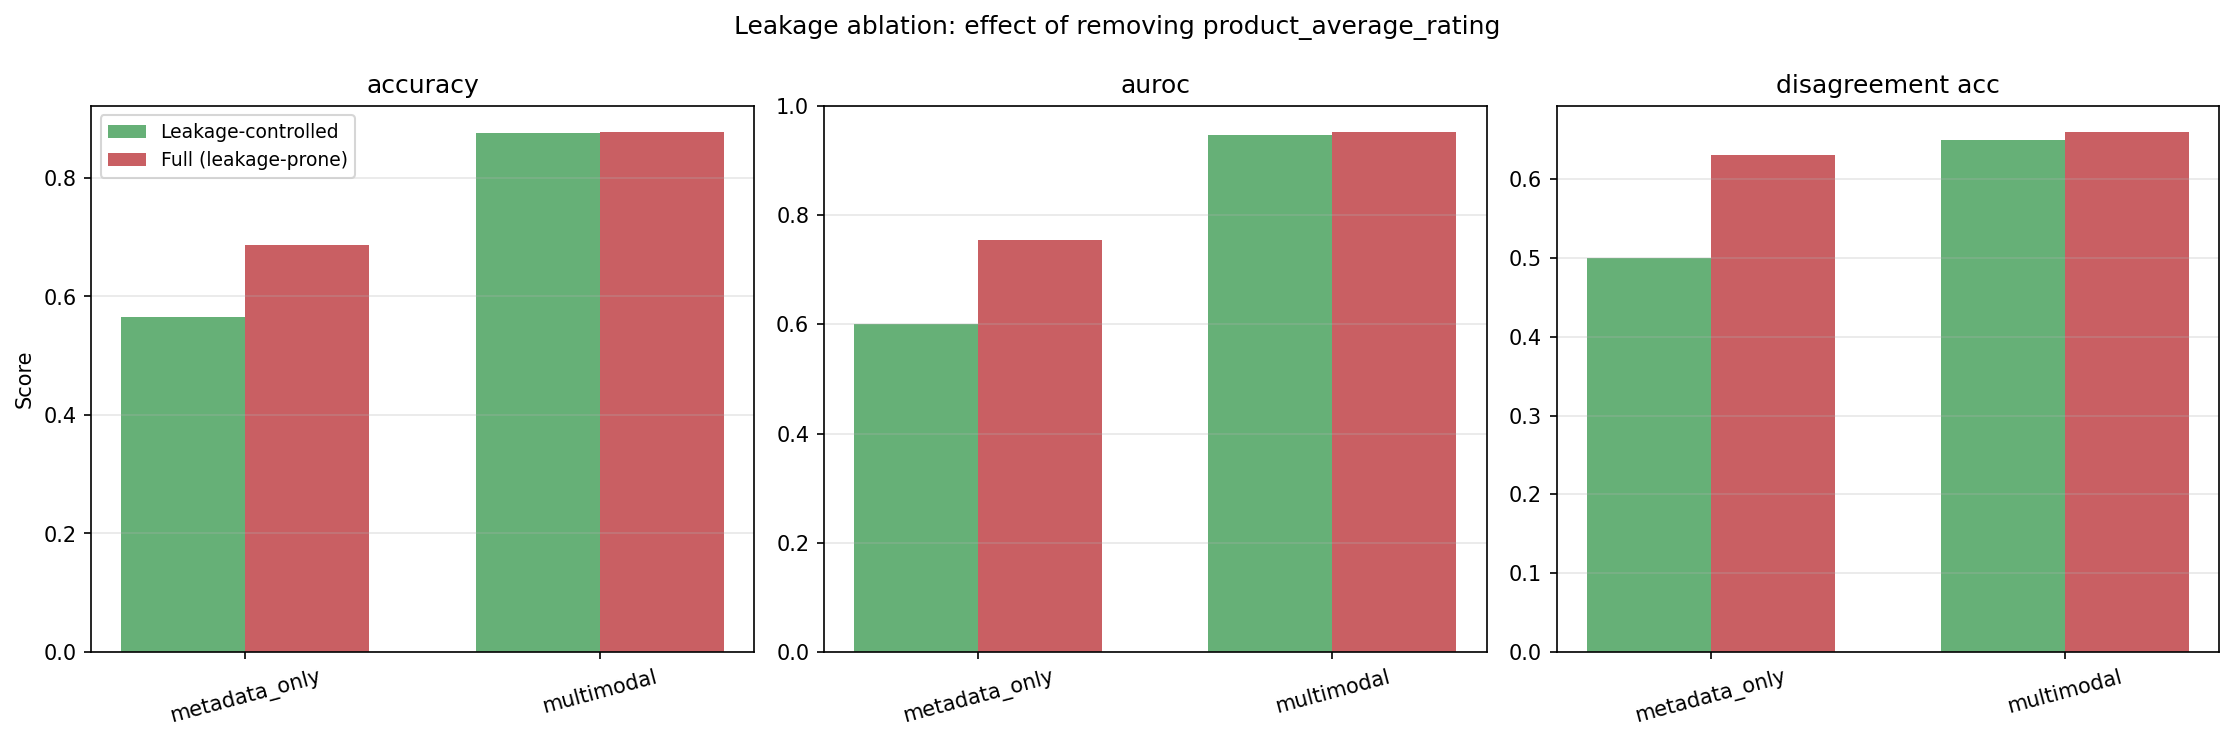
\includegraphics[width=0.95\textwidth]{pstat232_leakage_ablation.png}
\caption{Leakage ablation across accuracy, AUROC, and disagreement accuracy.
Green = leakage-controlled, red = full (leaky) feature set.}
\label{fig:leakage}
\end{figure}

\section{Methods}
\label{sec:methods}

\paragraph{Models (ERM estimators).}
\emph{Text-only}: $\ell_2$-regularized logistic regression on frozen
sentence-transformer (\texttt{all-MiniLM-L6-v2}) embeddings. \emph{Metadata-only}:
gradient-boosted trees (XGBoost, 200 estimators, depth 6) on standardized,
train-fit-imputed metadata. \emph{Multimodal}: an early-fusion MLP
($[\text{text}\,\Vert\,\text{meta}] \to 256 \to 64 \to 2$, ReLU, dropout $0.2$),
trained $15$ epochs with Adam and validation-accuracy early stopping.
\emph{Disagreement-aware}: identical architecture trained on the reweighted risk
($\omega=5$). All standardization and imputation statistics are fit on the
training split only.

\paragraph{Calibration.}
Temperature scaling fits a single scalar $T>0$ that rescales logits
$z \mapsto z/T$; we fit $T$ on the validation set by minimizing NLL (a proper
scoring rule, smooth in $T$) using bounded scalar optimization. ECE uses
$10$ equal-width bins.

\paragraph{Resampling inference.}
For a functional $\hat\phi$ we draw $B=2000$ nonparametric bootstrap resamples of
the test set and report the $2.5\%/97.5\%$ percentile interval. For paired model
comparisons we resample \emph{indices once per replicate} and difference the two
models' metrics on the same resample, giving a two-sided bootstrap $p$-value; we
report McNemar's continuity-corrected $\chi^2$ test alongside for accuracy.

\section{Disagreement-Aware Empirical Risk}
\label{sec:da-erm}

Table~\ref{tab:main} reports the primary leakage-controlled results.
Standard fusion ERM achieves the best overall accuracy ($0.876$) and AUROC
($0.947$), but its accuracy on the disagreement stratum is far lower ($0.649$),
exposing the conditional-risk gap. Reweighting the ERM objective toward
disagreement samples ($\omega=5$) raises disagreement accuracy to $0.663$ and
disagreement $F_1$ markedly, but \emph{shifts} risk: overall accuracy falls to
$0.862$ and overall ECE rises to $0.072$. This is the canonical bias--variance /
risk-reallocation trade-off made explicit: upweighting a subpopulation in the
empirical risk improves conditional performance there at a measurable global
cost.

\begin{table}[t]
\centering
\caption{Primary leakage-controlled results on the \texttt{All\_Beauty} test set
($n=3001$; disagreement $n=368$), seed 42. Best in each column in bold.}
\label{tab:main}
\begin{tabular}{lrrrrr}
\toprule
Model & Accuracy & Disagree.\ acc. & AUROC & ECE & Brier \\
\midrule
Text-only             & 0.873 & 0.641 & 0.943 & 0.028 & 0.093 \\
Metadata-only (LC)    & 0.566 & 0.500 & 0.600 & 0.050 & 0.245 \\
Multimodal (LC)       & \textbf{0.876} & 0.649 & \textbf{0.947} & \textbf{0.026} & \textbf{0.090} \\
Disagreement-aware (LC) & 0.862 & \textbf{0.663} & 0.936 & 0.072 & 0.108 \\
\bottomrule
\end{tabular}
\end{table}

\begin{figure}[t]
\centering
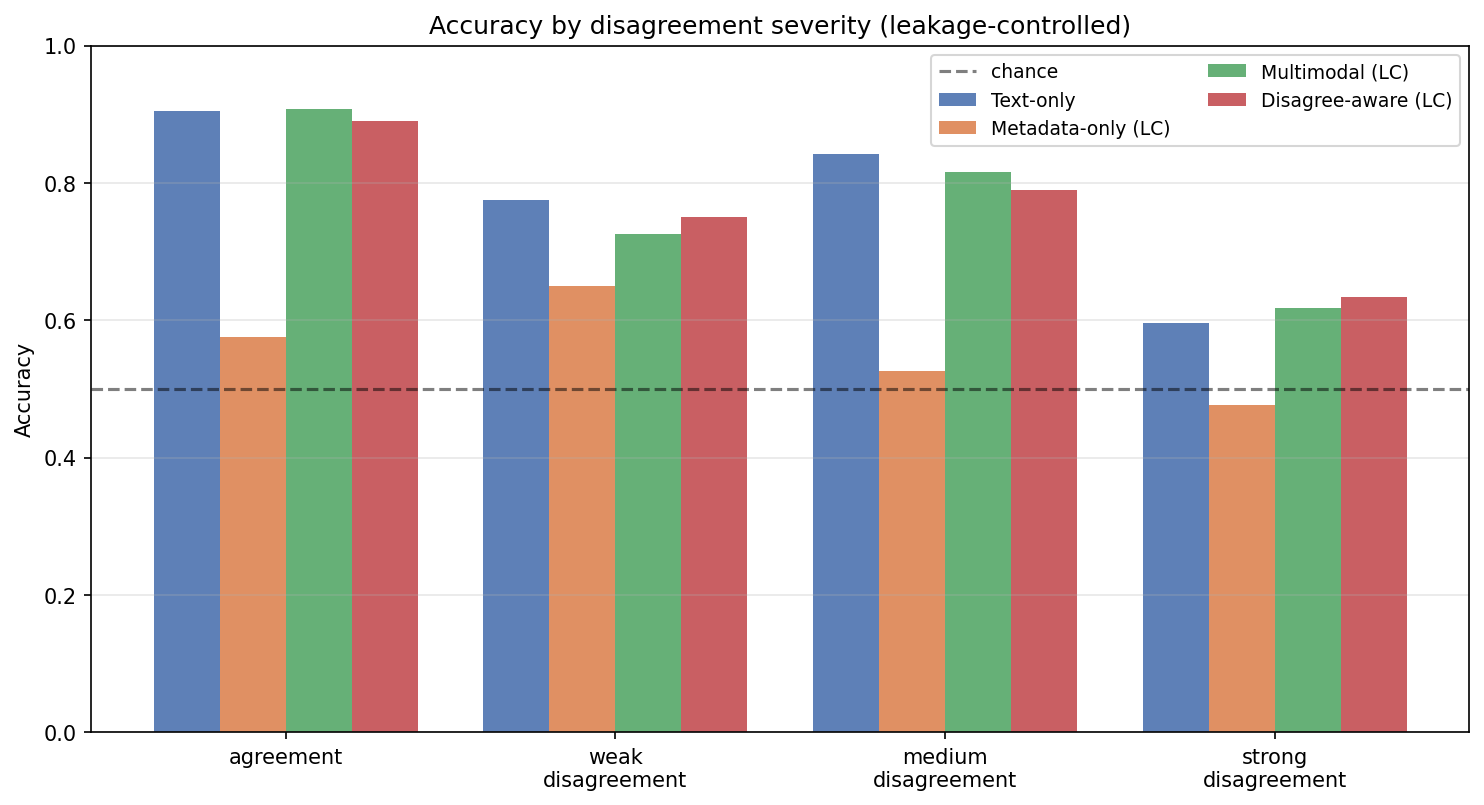
\includegraphics[width=0.8\textwidth]{pstat232_accuracy_by_disagreement.png}
\caption{Accuracy by disagreement severity. All models degrade monotonically
from agreement to strong disagreement; the disagreement-aware model trades a
little agreement accuracy for gains in the conflict strata.}
\label{fig:acc-disagree}
\end{figure}

\section{Calibration and Uncertainty Quantification}
\label{sec:calibration}

\paragraph{Group-conditional temperature scaling.}
We test whether miscalibration is homogeneous. Define an \emph{inference-time}
conflict proxy that uses only model outputs (never the label):
\[
\text{conflict}_i = \big(\hat y^{\text{text}}_i \neq \hat y^{\text{meta}}_i\big)
\;\vee\;
\big(|\hat p^{\text{text}}_i - \hat p^{\text{meta}}_i| > \tau\big),
\qquad \tau = 0.5 .
\]
We fit one global temperature $T_{\text{global}}$ on all validation data, and two
separate temperatures $T_{\text{conflict}}, T_{\text{non}}$ on the validation
conflict / non-conflict subsets, then apply each to the matching test subset.
Temperatures are frozen after validation, so there is no test leakage in the
calibration step.

\begin{table}[t]
\centering
\caption{Group-conditional calibration of the leakage-controlled fusion model
($\tau=0.5$, NLL objective). Temperatures: $T_{\text{global}}=1.18$,
$T_{\text{conflict}}=1.24$, $T_{\text{non}}=1.14$. Lower ECE/NLL/Brier is better;
accuracy is unchanged by temperature (a sanity check).}
\label{tab:groupcal}
\begin{tabular}{llrrrr}
\toprule
Method & Group & ECE & NLL & Brier & $n$ \\
\midrule
\multirow{3}{*}{Uncalibrated}
 & All         & 0.0262 & 0.2952 & 0.0900 & 3001 \\
 & Non-conflict& 0.0266 & 0.2649 & 0.0803 & 1676 \\
 & Conflict    & 0.0338 & 0.3335 & 0.1022 & 1325 \\
\midrule
\multirow{3}{*}{Global $T$}
 & All         & 0.0146 & 0.2915 & 0.0893 & 3001 \\
 & Non-conflict& 0.0157 & 0.2635 & 0.0799 & 1676 \\
 & Conflict    & \textbf{0.0244} & 0.3270 & 0.1012 & 1325 \\
\midrule
\multirow{3}{*}{Group-conditional $T$}
 & All         & 0.0160 & \textbf{0.2912} & \textbf{0.0893} & 3001 \\
 & Non-conflict& \textbf{0.0137} & \textbf{0.2632} & \textbf{0.0799} & 1676 \\
 & Conflict    & 0.0252 & 0.3266 & 0.1011 & 1325 \\
\bottomrule
\end{tabular}
\end{table}

Table~\ref{tab:groupcal} and Figure~\ref{fig:groupcal} give a nuanced,
\emph{honest} result. First, the conflict subset is genuinely less calibrated
than the non-conflict subset before any scaling (ECE $0.034$ vs.\ $0.027$),
confirming heterogeneity. Second, the fitted temperatures differ by group
($T_{\text{conflict}}=1.24 > T_{\text{non}}=1.14$), i.e.\ the model is
\emph{more} over-confident under conflict, exactly as the theory predicts. Third,
however, group-conditional scaling beats global scaling only on the non-conflict
group ($0.0137$ vs.\ $0.0157$ ECE) and on overall NLL; on the conflict subset the
global temperature is marginally better. The practical lesson is that once
leakage is controlled the fusion model is already well-calibrated, so the
\emph{room} for a group-conditional fix is small. This directly contrasts with
the leaky configuration, where conflict-driven miscalibration is large
(Table~\ref{tab:leakage}, full-feature fusion ECE $0.062$); leakage manufactures
much of the calibration pathology.

\begin{figure}[t]
\centering
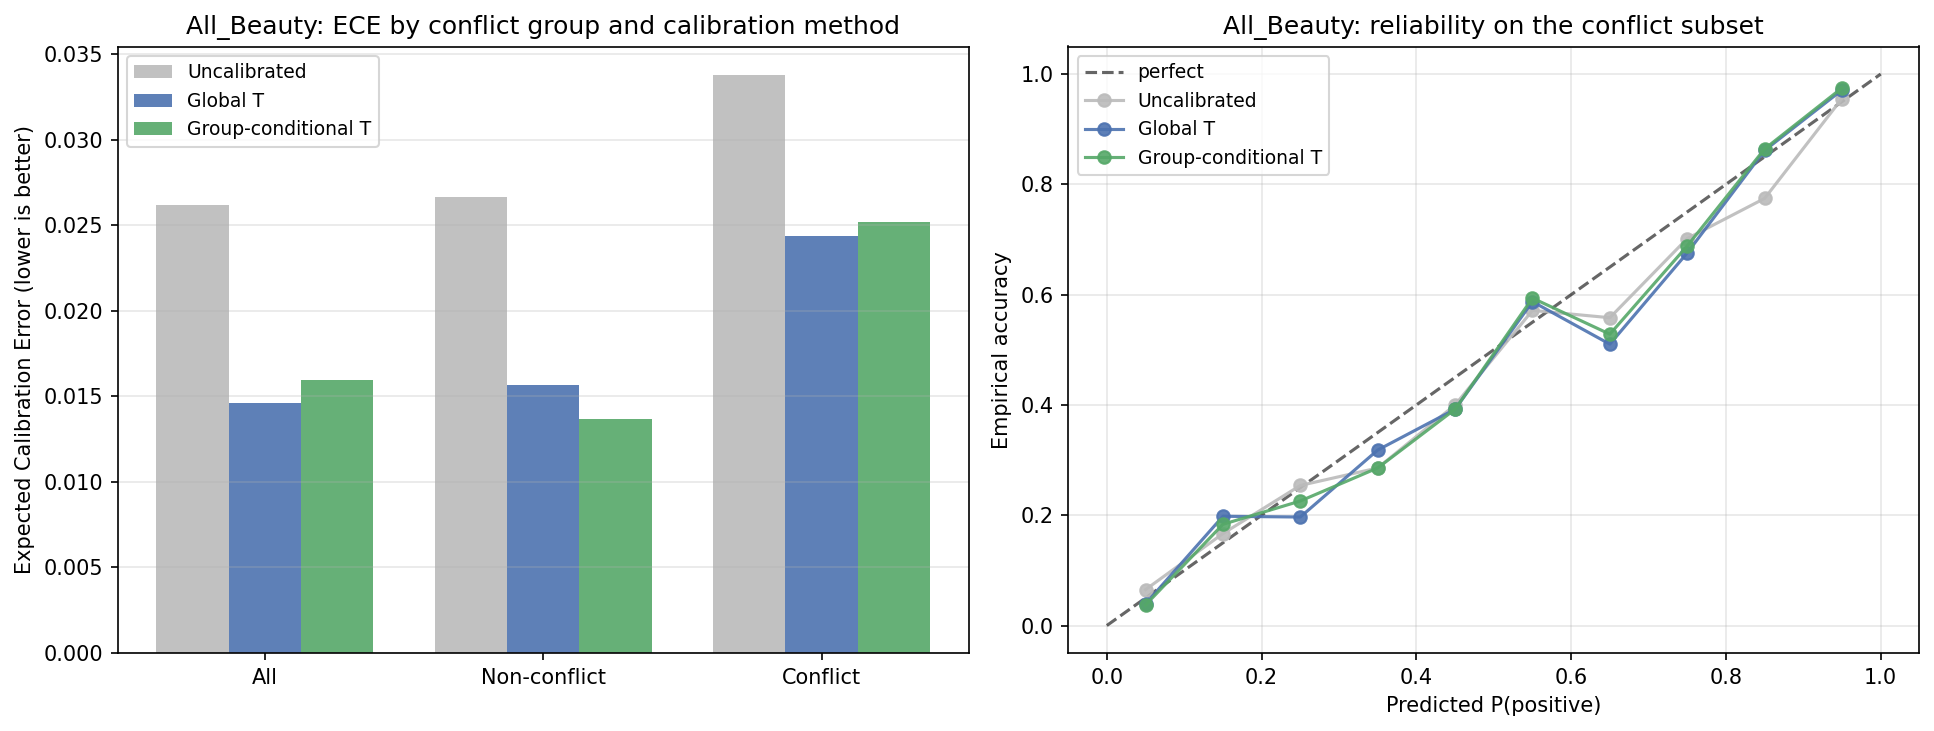
\includegraphics[width=\textwidth]{pstat232_group_calibration.png}
\caption{Left: ECE by conflict group and calibration method. Right: reliability
diagram on the conflict subset. Group-conditional scaling primarily helps the
non-conflict group.}
\label{fig:groupcal}
\end{figure}

\begin{figure}[t]
\centering
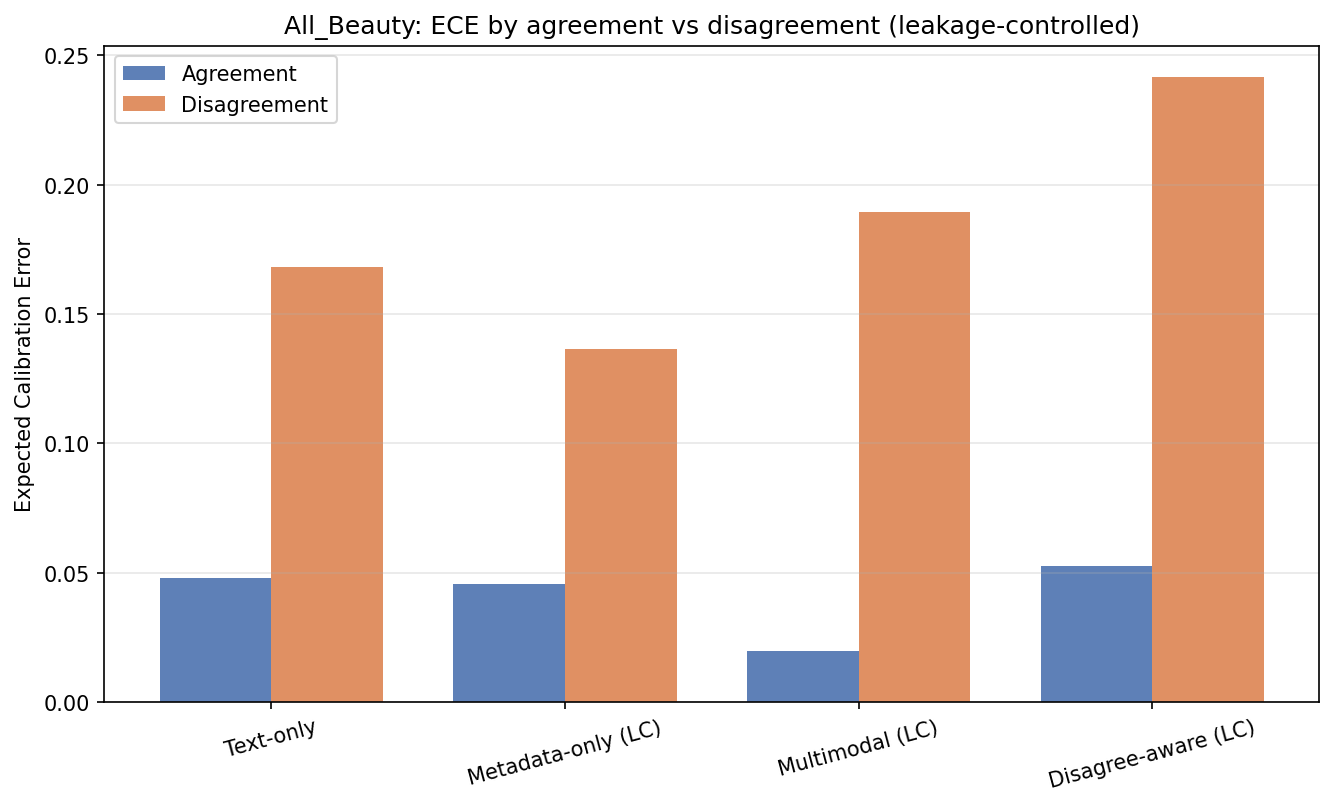
\includegraphics[width=0.72\textwidth]{pstat232_calibration_by_group.png}
\caption{ECE by agreement vs.\ disagreement for each model (leakage-controlled).
Every model is worse calibrated on the disagreement stratum.}
\label{fig:cal-by-group}
\end{figure}

\paragraph{Selective prediction.}
Figure~\ref{fig:selective} traces accuracy against coverage as we abstain on the
least-confident predictions. The fusion model's accuracy rises sharply with
abstention on the overall and agreement populations but improves only weakly on
the disagreement population, quantifying how little usable confidence signal
exists exactly where conflict occurs.

\begin{figure}[t]
\centering
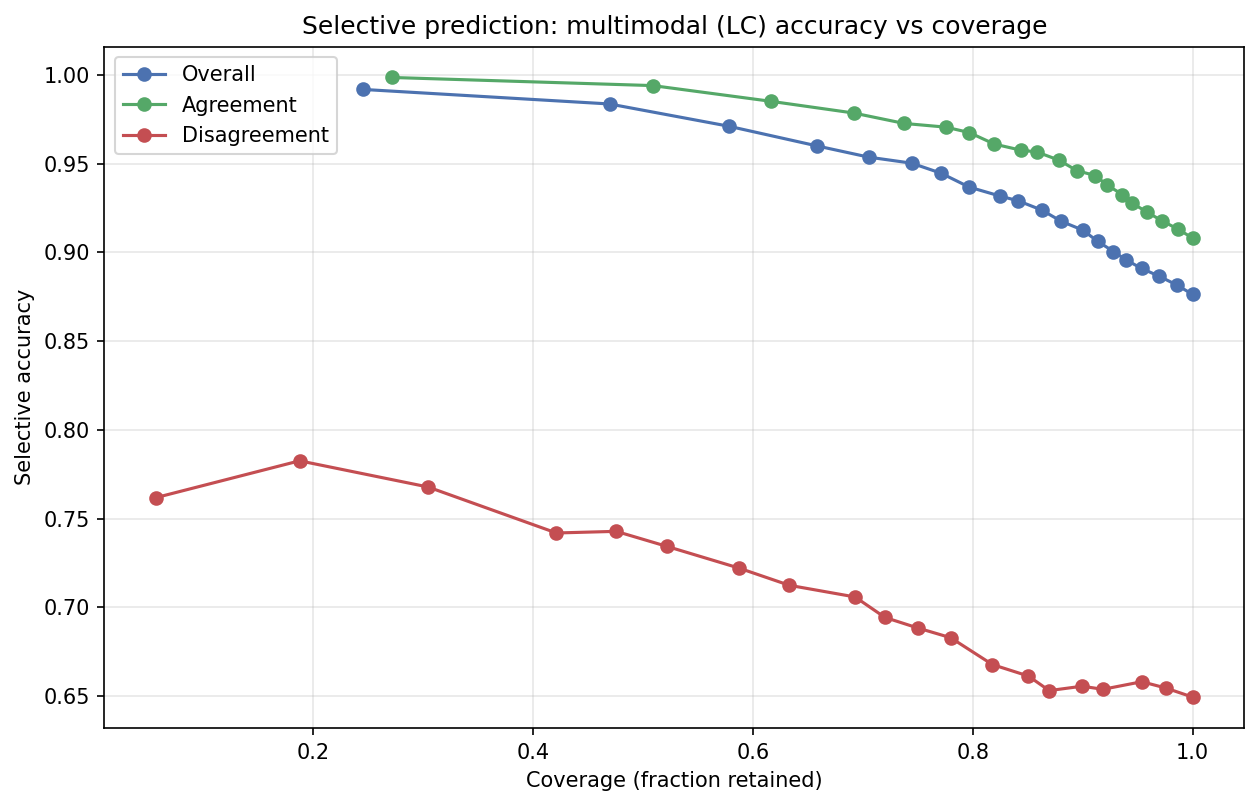
\includegraphics[width=0.72\textwidth]{pstat232_selective_prediction.png}
\caption{Selective accuracy vs.\ coverage for the leakage-controlled fusion
model. Confidence-based abstention helps far more under agreement than under
disagreement.}
\label{fig:selective}
\end{figure}

\section{Experiments}
\label{sec:experiments}

All experiments run offline from the materialized canonical pool and cached
embeddings; the pipeline is four scripts (Section~\ref{sec:repro}). The primary
configuration is \texttt{All\_Beauty}, seed $42$, leakage-controlled metadata,
$B=2000$ bootstrap resamples, conflict threshold $\tau=0.5$, and an NLL
temperature-fitting objective. The leakage ablation additionally trains
full-feature metadata and fusion models on the identical split.

\subsection{Reproducibility}
\label{sec:repro}
The entire PSTAT 232 pipeline runs offline from the materialized pool via four
scripts (and the convenience target \texttt{make pstat232}):
\begin{enumerate}[leftmargin=*,nosep]
  \item \texttt{python scripts/pstat232\_leakage\_controlled\_main.py --category All\_Beauty --seed 42}
  \item \texttt{python scripts/pstat232\_group\_conditional\_calibration.py --category All\_Beauty --tau 0.5}
  \item \texttt{python scripts/pstat232\_resampling\_inference.py --category All\_Beauty --n-boot 2000}
  \item \texttt{python scripts/pstat232\_make\_figures.py --category All\_Beauty}
\end{enumerate}
Step~1 persists per-sample validation and test predictions that steps 2--4
consume, so the calibration, inference, and figure steps require no retraining.

\section{Results}
\label{sec:results}

\paragraph{Resampling inference.}
Table~\ref{tab:ci} reports bootstrap $95\%$ CIs for the headline metrics. The
fusion and text-only intervals overlap heavily on accuracy, foreshadowing the
paired tests.

\begin{table}[t]
\centering
\caption{Nonparametric bootstrap ($B=2000$) point estimates and $95\%$
percentile CIs on the \texttt{All\_Beauty} test set.}
\label{tab:ci}
\begin{tabular}{llrr}
\toprule
Model & Metric (subset) & Estimate & 95\% CI \\
\midrule
Text-only          & Accuracy (overall)      & 0.873 & [0.860, 0.884] \\
Multimodal (LC)    & Accuracy (overall)      & 0.876 & [0.864, 0.888] \\
Metadata-only (LC) & Accuracy (overall)      & 0.566 & [0.548, 0.584] \\
Multimodal (LC)    & Accuracy (disagreement) & 0.649 & [0.601, 0.698] \\
Multimodal (LC)    & AUROC (overall)         & 0.947 & [0.940, 0.955] \\
Multimodal (LC)    & ECE (overall)           & 0.026 & [0.020, 0.039] \\
\bottomrule
\end{tabular}
\end{table}

\paragraph{Paired comparisons.}
Table~\ref{tab:paired} is the inferential core. Fusion is \emph{not}
statistically better than text-only either overall (paired bootstrap $p=0.42$,
McNemar $p=0.42$) or on the disagreement subset ($p=0.69$): the $+0.4$~pp
accuracy ``gain'' is within sampling noise. Fusion \emph{is} overwhelmingly
better than the leakage-controlled metadata model ($p<0.001$). The
disagreement-aware model is significantly \emph{worse} overall ($\Delta=-0.015$,
$p=0.002$) and its disagreement-subset improvement ($\Delta=+0.014$) is not
significant ($p=0.52$). Thus, with honest uncertainty, the headline ``fusion
helps'' claim does not survive on this category, and the mitigation buys
conditional accuracy at a real, significant global cost.

\begin{table}[t]
\centering
\caption{Paired comparisons: $\Delta = \text{metric}(A)-\text{metric}(B)$,
two-sided bootstrap $p$, and McNemar $p$ (accuracy only).}
\label{tab:paired}
\begin{tabular}{lllrrr}
\toprule
$A$ vs.\ $B$ & Subset & Metric & $\Delta$ & boot $p$ & McNemar $p$ \\
\midrule
Multimodal vs.\ Text       & overall      & acc & $+0.004$ & 0.42 & 0.42 \\
Multimodal vs.\ Text       & disagreement & acc & $+0.008$ & 0.69 & 0.76 \\
Multimodal vs.\ Metadata   & overall      & acc & $+0.311$ & $<0.001$ & $<0.001$ \\
Multimodal vs.\ Metadata   & disagreement & acc & $+0.149$ & $<0.001$ & $<0.001$ \\
Disagree-aware vs.\ Multimodal & overall  & acc & $-0.015$ & 0.002 & 0.002 \\
Disagree-aware vs.\ Multimodal & disagreement & acc & $+0.014$ & 0.52 & 0.55 \\
\bottomrule
\end{tabular}
\end{table}

\section{Interpretation}
\label{sec:interpretation}

Three computational-statistics conclusions emerge. (1) \textbf{Leakage
dominates apparent metadata skill.} A single product-level aggregate accounts for
most of the metadata model's measured accuracy and AUROC and, more subtly,
inflates fusion miscalibration; controlling it is essential for valid inference.
(2) \textbf{The fusion advantage is not significant under resampling.} On the
leakage-controlled task, the fusion ERM solution is statistically tied with a
text-only logistic regression---more parameters and a second modality do not buy
a detectable accuracy gain, and the cost of that complexity is real.
(3) \textbf{Miscalibration is heterogeneous but mild after leakage control.} The
conflict region is measurably less calibrated and warrants a larger temperature,
yet a global temperature already removes most of the error; the
group-conditional estimator helps chiefly on the non-conflict majority. The
strong conflict miscalibration observed in the full-feature setting was largely a
side-effect of leakage.

\section{Limitations}
\label{sec:limitations}

\begin{itemize}[leftmargin=*,nosep]
  \item \textbf{Disagreement is a proxy.} The conflict stratum is defined by a
        pretrained sentiment model versus the rating-derived label, so it is
        enriched for hard or mislabeled reviews rather than a clean
        ground-truth conflict signal.
  \item \textbf{Single primary category and seed.} Headline numbers use
        \texttt{All\_Beauty}, seed $42$. Four other categories are materialized
        for sensitivity runs, but the primary inferential claims are
        category-specific; cross-category replication is future work.
  \item \textbf{Calibration sample size.} The conflict test subset, while large
        in this category, is smaller than the non-conflict subset, so the
        conflict-group temperature is fit on fewer points and its ECE estimates
        carry wider uncertainty.
  \item \textbf{Bootstrap caveats.} Percentile intervals can be biased for ECE
        (a binned, non-smooth functional); we report them as indicative rather
        than exact.
\end{itemize}

\section{Conclusion}
\label{sec:conclusion}

This computational study of multimodal disagreement yields sharper, more honest
conclusions than a leaderboard-style comparison. Empirical risk
decomposition exposes a conditional-risk gap under conflict; reweighted ERM
reallocates rather than eliminates that risk; resampling inference shows the
fusion advantage is within sampling noise once leakage is controlled; and
group-conditional calibration confirms heterogeneous miscalibration while
revealing that most of the apparent calibration pathology under the leaky
configuration is a leakage artifact. The accompanying scripts reproduce every
figure and table end-to-end from materialized data.

\begin{thebibliography}{9}
\bibitem{guo2017calibration} C.\ Guo, G.\ Pleiss, Y.\ Sun, K.\ Q.\ Weinberger.
  On Calibration of Modern Neural Networks. 2017.
\bibitem{efron1994bootstrap} B.\ Efron, R.\ Tibshirani.
  \emph{An Introduction to the Bootstrap}. Chapman \& Hall, 1994.
\bibitem{dietterich1998} T.\ G.\ Dietterich.
  Approximate Statistical Tests for Comparing Supervised Classification
  Learning Algorithms. \emph{Neural Computation}, 10(7), 1998.
\bibitem{reimers2019sbert} N.\ Reimers, I.\ Gurevych.
  Sentence-BERT: Sentence Embeddings using Siamese BERT-Networks. 2019.
\bibitem{hovy2021} D.\ Hovy, S.\ Prabhumoye.
  Five sources of bias in natural language processing.
  \emph{Language and Linguistics Compass}, 2021.
\bibitem{kaufman2012leakage} S.\ Kaufman, S.\ Rosset, C.\ Perlich.
  Leakage in Data Mining. \emph{ACM TKDD}, 6(4), 2012.
\end{thebibliography}

\end{document}
